\documentclass[11pt]{article}
\usepackage[margin=1in]{geometry}
\usepackage{iftex}
\ifXeTeX
  \usepackage{fontspec}
  \setmainfont{Latin Modern Roman}
  \usepackage{xeCJK}
  \setCJKmainfont{Noto Serif CJK SC}
  \setCJKsansfont{Noto Sans CJK SC}
  \setCJKmonofont{Noto Sans Mono CJK SC}
  \newCJKfontfamily\zhfont{Noto Serif CJK SC}
\else
  \usepackage[T1]{fontenc}
  \usepackage{lmodern}
\fi
\usepackage{microtype}
\usepackage{amsmath,amssymb,amsthm,mathtools}
\usepackage{booktabs,array,longtable,tabularx}
\usepackage[dvipsnames]{xcolor}
\usepackage{tikz}
\usetikzlibrary{arrows.meta,positioning,calc,shapes.geometric}
\usepackage[numbers,sort&compress]{natbib}
\usepackage{hyperref}
\usepackage{xurl}
\usepackage{enumitem}
\usepackage{xspace}

\definecolor{FlowBlue}{HTML}{0072B2}
\definecolor{FlowTeal}{HTML}{009E73}
\definecolor{FlowOrange}{HTML}{E69F00}
\definecolor{FlowRed}{HTML}{D55E00}
\hypersetup{colorlinks=true,linkcolor=MidnightBlue,citecolor=ForestGreen,
 urlcolor=BrickRed,pdftitle={Which Operator Owns the Zeta?},pdfauthor={Liang Wang}}
\urlstyle{same}
\setlength{\emergencystretch}{3em}

\newtheorem{theorem}{Theorem}
\newtheorem{proposition}[theorem]{Proposition}
\newtheorem{corollary}[theorem]{Corollary}
\newtheorem{lemma}[theorem]{Lemma}
\theoremstyle{remark}\newtheorem{remark}[theorem]{Remark}
\newcommand{\R}{\mathbb R}
\newcommand{\Q}{\mathbb Q}
\newcommand{\Z}{\mathbb Z}
\newcommand{\F}{\mathbb F}
\newcommand{\Hh}{\mathcal H}
\newcommand{\D}{\mathcal D}
\newcommand{\Tr}{\operatorname{Tr}}
\newcommand{\Ran}{\operatorname{Ran}}
\newcommand{\e}{\mathrm e}
\newcommand{\proved}{\textsf{PROVED}\xspace}
\newcommand{\failed}{\textsf{FAIL}\xspace}
\newcolumntype{Y}{>{\raggedright\arraybackslash}X}

\title{\textbf{Which Operator Owns the Zeta?}\\
Koopman and Frobenius Ledgers of an Arithmetic Suspension}
\author{Liang Wang\\
\small School of Artificial Intelligence and Automation,\\[-2pt]
\small Huazhong University of Science and Technology, Wuhan 430074, P.R. China\\
\small \texttt{wangliang.f@gmail.com}}
\date{13 August 2026}

\begin{document}
\maketitle

\begin{abstract}
An arithmetic parent can generate an exact orbit zeta and a natural
self-adjoint flow operator without making the two constructions one spectral
determinant.  We prove this distinction for the constant-roof Frobenius
suspension of \(\mathbb P^1/\mathbb F_2\).  Closed points, primitive suspension
circles, point counts, and graded \(\ell\)-adic Frobenius traces form one exact
native ledger:
\[
 \sum_{d\mid n}d a_d=1+2^n
 \quad\text{and}\quad
 Z(X,t)=\frac1{(1-t)(1-2t)}.
\]
The determinant owner is Frobenius on finite-dimensional graded \(\ell\)-adic
cohomology.  The natural Koopman owner of suspension time is instead the
self-adjoint periodic derivative \(A_K\) on the Hilbert direct sum of all
closed-point circles.  Its point spectrum is
\((2\pi/\log2)\mathbb Q\), every eigenvalue has countably infinite
multiplicity, and its full and essential spectra equal \(\mathbb R\).  Hence
its resolvent is noncompact and its Gaussian heat operator is not trace class.
The two operators are not unitarily equivalent, and adjoining any
finite-dimensional realization of Frobenius to \(A_K\) preserves the
essential-spectrum obstruction.  The substitution \(t=2^{-s}\) merely lifts
the two native factors to pole lattices on \(\operatorname{Re}s=0,1\); it does
not create a self-adjoint energy spectrum.  This is an exact same-parent
Lefschetz positive control and a frozen-object Route-B obstruction, not a
universal no-go theorem for future cohomological flows.
\end{abstract}

\ifPDFTeX\else
\begin{center}{\zhfont\bfseries 摘要}\end{center}
{\zhfont
同一个算术母体可以同时产生精确的轨道 zeta 与自然的自伴流算子，但这并不
意味着二者属于同一个谱行列式。本文在
\(\mathbb P^1/\mathbb F_2\) 的常值屋顶 Frobenius 悬挂流上严格证明这种
区别。闭点、本原悬挂圆周、点计数与分次 \(\ell\)-进 Frobenius 迹构成一个
精确的有限域账本：\(\sum_{d\mid n}d a_d=1+2^n\)，且
\(Z(X,t)=((1-t)(1-2t))^{-1}\)。这个行列式的拥有者是有限维分次
\(\ell\)-进上同调上的 Frobenius。悬挂时间的自然 Koopman 拥有者则是所有
闭点圆周 Hilbert 直和上的周期导数 \(A_K\)。该算子自伴，点谱为
\((2\pi/\log2)\mathbb Q\)，每个特征值均具有可数无穷重数，全谱与本质谱
均为 \(\mathbb R\)；因此预解算子不紧，Gaussian 热算子也非迹类。两个
算子不可能酉等价；把 Frobenius 的任意有限维实现直和到 \(A_K\) 上，仍然
保留本质谱阻碍。变量代换 \(t=2^{-s}\) 只把两个有限域因子提升成
\(\operatorname{Re}s=0,1\) 上的极点格，并不会产生新的自伴能谱。该结果是
精确的同母体 Lefschetz 正控与冻结对象上的 Route-B 阻碍，而不是对未来
所有上同调流的普遍不可行定理。
}
\fi

\medskip
\noindent\textbf{Keywords:} Frobenius suspension; Hasse--Weil zeta;
Lefschetz trace; Koopman generator; operator ownership; essential spectrum.

\section{Introduction}

Scalar equality is weaker than operator identity.  This is especially easy
to overlook when several constructions arise from the same arithmetic
scheme.  Closed points of a finite-field variety give an Euler product; their
geometric Frobenius cycles give a suspension flow; and étale cohomology gives
an exact graded determinant.  The first two papers in this branch established
an exact finite-field orbit-zeta positive control and then classified its
canonical Koopman lift.  The present paper asks which operator actually owns
the determinant.

For the frozen example \(X=\mathbb P^1_{\F_2}\), all three classical ledgers
are exact.  Deligne's trace and determinant formulas identify the owner of
the native zeta as Frobenius on graded étale cohomology
\citep{Deligne1974}.  Koopman's construction, Stone's theorem, and the
orthogonal-sum theorem independently identify a complete self-adjoint
generator of suspension time \citep{Koopman1931,Stone1932,Teschl2009}.
Those are positive results, but they belong to different analytic operators.

The distinction is decisive for Route B.  A certificate cannot take
self-adjointness from the Koopman derivative and a determinant from
cohomological Frobenius unless an operator-level morphism and trace theorem
transport both properties.  Here an explicit spectral comparison rules out
that identification for the frozen pair.  It does not rule out a new
cohomological flow, anisotropic transfer operator, or source-derived bridge.

\begin{figure}[t]
\centering
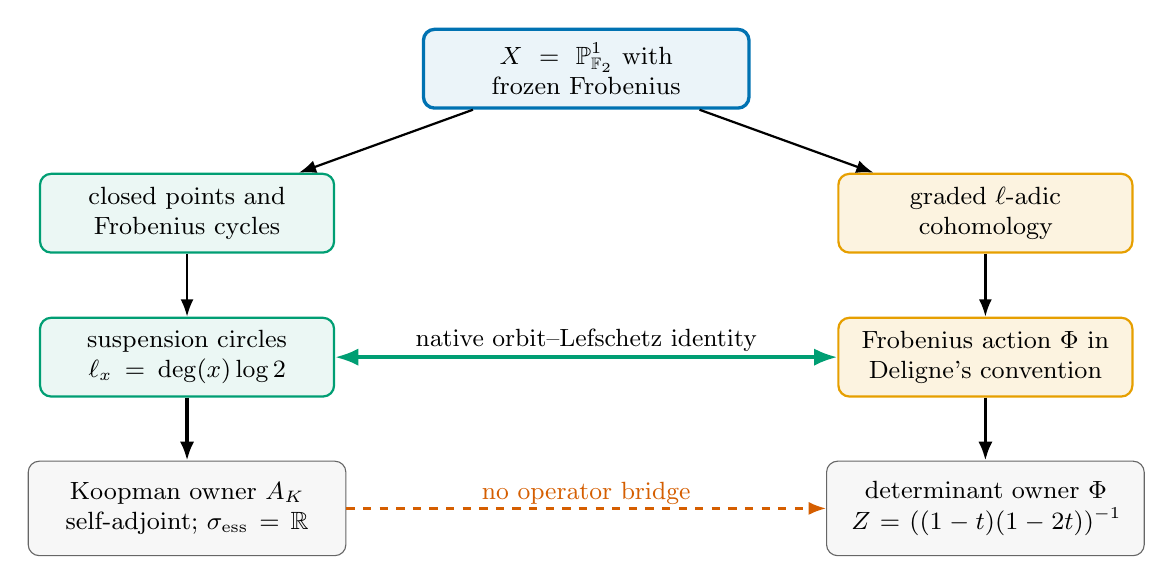
\begin{tikzpicture}[
  >=Latex,
  node distance=8mm and 11mm,
  every node/.style={font=\small,align=center},
  parent/.style={draw=FlowBlue,very thick,rounded corners,fill=FlowBlue!8,
    text width=39mm,minimum height=10mm},
  orbit/.style={draw=FlowTeal,thick,rounded corners,fill=FlowTeal!8,
    text width=35mm,minimum height=10mm},
  coho/.style={draw=FlowOrange,thick,rounded corners,fill=FlowOrange!12,
    text width=35mm,minimum height=10mm},
  result/.style={draw=black!60,rounded corners,fill=black!3,
    text width=38mm,minimum height=12mm},
  own/.style={-{Latex[length=2.4mm]},very thick},
  derive/.style={-{Latex[length=2.2mm]},thick},
  absent/.style={-{Latex[length=2.2mm]},thick,dashed,FlowRed}
]
\node[parent] (parent) {$X=\mathbb P^1_{\mathbb F_2}$\ with frozen Frobenius};
\node[orbit,below left=of parent] (cycles) {closed points and\ Frobenius cycles};
\node[coho,below right=of parent] (coho) {graded \(\ell\)-adic\ cohomology};
\node[orbit,below=of cycles] (circles) {suspension circles\ \(\ell_x=\deg(x)\log2\)};
\node[coho,below=of coho] (phi) {Frobenius action \(\Phi\)\ in Deligne's convention};
\node[result,below=of circles] (koop) {Koopman owner \(A_K\)\ self-adjoint; \(\sigma_{\rm ess}=\mathbb R\)};
\node[result,below=of phi] (det) {determinant owner \(\Phi\)\ \(Z=((1-t)(1-2t))^{-1}\)};

\draw[derive] (parent) -- (cycles);
\draw[derive] (parent) -- (coho);
\draw[derive] (cycles) -- (circles);
\draw[derive] (coho) -- (phi);
\draw[own] (circles) -- (koop);
\draw[own] (phi) -- (det);
\draw[FlowTeal,very thick,<->] (circles.east) -- node[above,text=black,
  fill=white,inner sep=1.5pt] {native orbit--Lefschetz identity} (phi.west);
\draw[absent] (koop.east) -- node[above,text=FlowRed,fill=white,
  inner sep=1pt] {no operator bridge} (det.west);
\end{tikzpicture}
\caption{One arithmetic parent has two different analytic operator owners.
The solid bridge is the exact native closed-point--cohomology identity.  The
dashed no-bridge arrow is not an impossibility claim for all future bridges; it
records that no identification exists for the two frozen operators.}
\label{fig:ownership}
\end{figure}


\section{Frozen parent and three typed ledgers}

Let
\[
 X=\mathbb P^1_{\F_2},\qquad
 S=X(\overline{\F}_2)_{\rm disc},\qquad F(a)=a^2,
 \qquad \tau=\log2.
\]
We use ``square-map Frobenius'' for \(F\); sources that distinguish
arithmetic and geometric Frobenius may use inverse conventions.  Inverting
the permutation reverses every finite cycle but preserves its degree and the
suspension lengths used below.

The mapping torus and vertical flow are
\[
 M_F=(S\times\R)/\Z,\qquad
 n\cdot(a,u)=(F^na,u-n\tau),\qquad
 \phi^t[a,u]=[a,u+t].
\]
Closed points are the finite Frobenius orbits on geometric points
\citep[Sec.~1.4]{Deligne1974}.  A closed point \(x\) of degree \(d_x\)
therefore gives the primitive circle
\[
 C_x=\R/(d_x\tau\Z),\qquad \ell_x=d_x\tau=\log N(x),
 \qquad M_F\cong\coprod_{x\in|X|}C_x.
\]
The coproduct topology is a disclosed modeling choice; it is not the scheme
topology.

Fix an auxiliary prime \(\ell\ne2\), and write
\[
 H^i_{\rm et}=H^i_{\rm et}(X_{\overline{\F}_2},\Q_\ell),\qquad
 \Phi=F^*:H^i_{\rm et}\longrightarrow H^i_{\rm et},
\]
where \(F^*\) is exactly the pullback convention in Deligne's
equations~(1.5.1)--(1.5.4).  In Deligne's Galois terminology this action
corresponds to geometric Frobenius, whereas the displayed point map remains
the square map \(a\mapsto a^2\).  This convention statement, rather than an
informal name, fixes every trace and determinant below.

Table~\ref{tab:owners} freezes the three ledgers.  A common parent is a real
provenance relation, but it is not an operator conjugacy.

\begin{table}[t]
\centering\small
\caption{The frozen ledgers and their operator owners.}
\label{tab:owners}
\begin{tabularx}{\textwidth}{@{}p{0.16\textwidth}p{0.22\textwidth}YY@{}}
\toprule
Ledger & Space/objects & Action or owner & Exact output\\
\midrule
Orbit & primitive circles \(C_x\) & repeats of lengths \(d_x\log2\) & closed-point Euler product\\
Koopman & \(\bigoplus_x L^2(C_x,w_xdu)\) & \(A_K=-i\,d/du\), periodic domain & self-adjoint time; dense essential spectrum\\
Cohomology & \(\bigoplus_iH^i_{\rm et}(X_{\overline{\F}_2},\Q_\ell)\) & graded Frobenius \(\Phi\) & exact Lefschetz trace and determinant\\
\bottomrule
\end{tabularx}
\end{table}

\section{Closed points in every degree}

Let \(a_d\) be the number of degree-\(d\) closed points of \(X\).  The
factorization of \(T^{2^n}-T\) as the product of all monic irreducible
polynomials whose degrees divide \(n\) gives
\(2^n=\sum_{d\mid n}dI_d\).  Möbius inversion therefore gives
\[
 a_1=3,\qquad
 a_d=\frac1d\sum_{e\mid d}\mu(e)2^{d/e}\quad(d>1).
\]

\begin{lemma}\label{lem:degrees}
For every integer \(d\ge1\), \(a_d>0\).
\end{lemma}
\begin{proof}
The degree-one points are \(0,1,\infty\).  For \(d\ge2\), discard all
positive summands except \(2^d\) and bound the others absolutely:
\[
 d a_d\ge 2^d-\sum_{\substack{e\mid d\\e\ge2}}2^{d/e}
 \ge2^d-\sum_{m=1}^{\lfloor d/2\rfloor}2^m
 =2^d-2^{\lfloor d/2\rfloor+1}+2>0.
\]
Since \(a_d\) is an integer, it is positive.
\end{proof}

Only existence, rather than the exponential size of \(a_d\), is needed for
the spectral obstruction.  One component in each positive degree already
produces all denominators infinitely often.

\section{Exact point, cycle, and cohomological traces}

\begin{theorem}[Three exact native ledgers]\label{thm:ledgers}
For every \(n\ge1\),
\begin{equation}
 \sum_{d\mid n}d a_d
 =\#\mathbb P^1(\F_{2^n})
 =1+2^n
 =\sum_i(-1)^i\Tr(\Phi^n\mid H^i_{\rm et}).
 \label{eq:three-traces}
\end{equation}
Consequently, as a formal series and analytically for \(|t|<1/2\),
\begin{equation}
 \begin{split}
 Z(X,t)
 &=\exp\!\left(\sum_{n\ge1}\frac{1+2^n}{n}t^n\right)\\
 &=\prod_{x\in|X|}(1-t^{d_x})^{-1}
 =\prod_i\det(1-t\Phi\mid H^i_{\rm et})^{(-1)^{i+1}}\\
 &=\frac1{(1-t)(1-2t)}.
 \end{split}\label{eq:graded-determinant}
\end{equation}
\end{theorem}

\begin{proof}
A primitive cycle of length \(d\) contributes all \(d\) of its points to
\(\operatorname{Fix}(F^n)\) exactly when \(d\mid n\), proving the first
equality.  The projective line over \(\F_{2^n}\) has \(2^n+1\) points.
Deligne's Lefschetz formula gives the final equality in
\eqref{eq:three-traces}, and his determinant formula identifies the graded
product in \eqref{eq:graded-determinant}
\citep[Eqs.~(1.5.1)--(1.5.4)]{Deligne1974}.  Equivalently, the two nonzero
graded trace eigenvalues are \(1\) and \(2\).  Applying
\(-\log(1-z)=\sum_{n\ge1}z^n/n\) proves the remaining identities and their
absolute convergence for \(|t|<1/2\).
\end{proof}

The theorem answers the native ownership question: the exact determinant is
the graded finite-dimensional cohomological determinant of \(\Phi\).  It is
not thereby a Fredholm or spectral-zeta determinant of the Koopman generator.
The Stacks trace chapter supplies an independent modern convention check;
Deligne remains the load-bearing primary source \citep{StacksTrace2026}.

\section{Complete Koopman owner of suspension time}

Choose arbitrary component constants \(0<w_x<\infty\) and define
\[
 \Hh_w=\bigoplus_{x\in|X|}L^2(C_x,w_xdu),\qquad
 (U_t^{(w)}f)_x(u)=f_x(u-t).
\]
Translation invariance gives a unitary group, and finite-component
approximation proves strong continuity.  This is the standard Koopman
pullback construction \citep{TerElstLemanczyk2017}.  The candidate uses the
Stone convention \(U_t^{(w)}=\e^{-itA_w}\).

Define
\[
 A_w=\bigoplus_x\left(-i\frac d{du}\right)_x
\]
on the complete graph domain
\begin{equation}
 \D(A_w)=\left\{f=(f_x):
 \begin{array}{l}
 f_x\in H^1_{\rm per}(0,d_x\log2)\text{ for every }x,\\
 \displaystyle\sum_xw_x\bigl(\|f_x\|_{L^2(du)}^2+
                   \|f_x'\|_{L^2(du)}^2\bigr)<\infty
 \end{array}\right\}.
 \label{eq:domain}
\end{equation}

\begin{theorem}[Complete self-adjoint generator]\label{thm:selfadjoint}
The operator \(A_w\) on \eqref{eq:domain} is self-adjoint and is the unique
Stone generator of \(U_t^{(w)}\).  All positive component-weight choices are
unitarily equivalent.
\end{theorem}
\begin{proof}
On a degree-\(d_x\) component, periodic Fourier series give the normalized
basis
\[
 e_{x,n}^{(w)}(u)=(w_xd_x\log2)^{-1/2}
   \e^{2\pi inu/(d_x\log2)},\qquad
 A_we_{x,n}^{(w)}=\frac{2\pi n}{d_x\log2}e_{x,n}^{(w)}.
\]
Thus each component is real multiplication on its maximal periodic
\(H^1\) domain.  The countable orthogonal-sum theorem gives self-adjointness
on exactly \eqref{eq:domain} \citep[Thm.~2.23]{Teschl2009}, and Stone's
theorem identifies the translation generator \citep[Thms.~5.1--5.2]{Teschl2009}.
Finally, \((W_wf)_x=\sqrt{w_x}f_x\) is a unitary map to the unweighted
space and commutes with translations and differentiation.
\end{proof}

This establishes a genuine complete operator and self-adjointness.  It does
not establish a suitable spectral type or an arithmetic trace.

\section{Exact Koopman spectral type}

\begin{theorem}[Dense and essential spectrum]\label{thm:spectrum}
For every positive component-weight family,
\begin{equation}
 \sigma_{\rm p}(A_w)=\frac{2\pi}{\log2}\Q,
 \qquad
 \sigma(A_w)=\sigma_{\rm ess}(A_w)=\R.
 \label{eq:spectrum}
\end{equation}
Every point eigenvalue has countably infinite multiplicity, and
\(\sigma_{\rm disc}(A_w)=\varnothing\).
\end{theorem}
\begin{proof}
Lemma~\ref{lem:degrees} and the component Fourier formula give
\[
 \bigcup_{d\ge1}\frac{2\pi}{d\log2}\Z
 =\frac{2\pi}{\log2}\Q.
\]
For a reduced rational \(a/b\), degrees \(kb\) and modes \(ka\),
\(k\ge1\), give mutually orthogonal eigenvectors with the same eigenvalue.
The basis is countable, so the multiplicity is countably infinite.  The
orthogonal-sum spectrum is the closure of the component spectra, hence
\(\R\).  Rational points already have infinite-dimensional eigenspaces.  At
an irrational \(\lambda\), choose rational eigenvalues \(\lambda_j\to\lambda\)
on mutually distinct components; their normalized eigenvectors are a
singular Weyl sequence.  Every real point is therefore essential.
\end{proof}

The Fourier eigenvectors form a complete basis, so every vector spectral
measure is pure point.  This is compatible with
\(\sigma_{\rm c}(A_w)=\R\setminus(2\pi/\log2)\Q\) in the set-theoretic
operator decomposition: the irrational points are non-eigenvalue
accumulation points with dense nonsurjective range.

\begin{corollary}[Compactness and heat obstruction]\label{cor:heat}
The resolvent of \(A_w\) is not compact.  Every interval of positive width
has infinite-rank spectral projection, and \(\e^{-tA_w^2}\) is not trace
class for any \(t>0\).  Deleting the zero eigenspace does not repair these
failures.
\end{corollary}
\begin{proof}
The zero Fourier mode on each of the countably many components gives an
infinite-dimensional kernel.  The resolvent acts by the same nonzero scalar
on that subspace, and the heat operator acts as the identity.  After deleting
the kernel, fix any nonzero rational eigenvalue; its infinite-dimensional
eigenspace gives the same argument.  Every positive-width interval contains
a rational eigenvalue of infinite multiplicity.
\end{proof}

\section{The operator-ownership theorem}

\begin{theorem}[Same parent, different analytic owners]\label{thm:owner}
For the frozen parent \((X,F)\):
\begin{enumerate}[label=(\roman*)]
\item \(A_w\) is the self-adjoint owner of suspension time;
\item \(\Phi\) is the owner of the exact native graded determinant
      \eqref{eq:graded-determinant};
\item no unitary equivalence identifies these two operators;
\item adjoining any finite-dimensional complex realization of \(\Phi\) to
      \(A_w\) leaves essential spectrum \(\R\), noncompact resolvent, and
      non-trace-class heat.
\end{enumerate}
Thus a Route-B certificate cannot combine self-adjointness from \(A_w\) with
the trace or determinant of \(\Phi\) without proving a new one-operator
bridge.
\end{theorem}
\begin{proof}
The first two claims are Theorems~\ref{thm:selfadjoint} and
\ref{thm:ledgers}.  The Koopman owner acts on an infinite-dimensional complex
Hilbert space and has spectrum \(\R\); the cohomological owner is a
two-dimensional graded \(\Q_\ell\)-linear action with eigenvalue ledger
\(\{1,2\}\).  They are not even operators over the same scalar field as
frozen, and after any noncanonical complex realization their spectra exclude
unitary equivalence.  A finite-dimensional direct summand cannot remove the
infinite-dimensional eigenspaces in Theorem~\ref{thm:spectrum}, so every
claim in Corollary~\ref{cor:heat} persists.
\end{proof}

The theorem is object-specific.  A genuinely new cohomological flow,
anisotropic space, coupling, or boundary condition must be frozen as a new
candidate and re-audited; it is not ruled out here.

\section{The exponential lift is a variable preimage}

\begin{proposition}[Lifted native divisor]\label{prop:lift}
For \(\alpha\in\{1,2\}\), the solutions of
\(1-\alpha2^{-s}=0\) are
\[
 s=\frac{\log\alpha+2\pi ik}{\log2},\qquad k\in\Z.
\]
Consequently the two inverse factors have pole lattices on
\(\operatorname{Re}s=0\) and \(\operatorname{Re}s=1\), with imaginary period
\(2\pi/\log2\).
\end{proposition}
\begin{proof}
The equation is \(\exp(\log\alpha-s\log2)=1\).  Solving modulo
\(2\pi i\Z\) and renaming the integer sign gives the formula.
\end{proof}

The infinitely many preimages arise because \(s\mapsto2^{-s}\) is periodic.
They are not new Frobenius eigenvalues or energies of \(A_w\), and their
divisor is not the completed Riemann \(\xi\) divisor.

\section{Same-object certificate and route decisions}

The orbit and cohomological ledgers pass a native same-parent certificate:
Deligne's theorem supplies a typed global trace and determinant, not merely a
coordinate splice.  The stronger single-operator certificate fails because
the self-adjoint and determinant owners differ.  Table~\ref{tab:routes}
records the two target scopes separately.

\begin{table}[t]
\centering\small
\caption{Frozen Route-A and limited Route-B decisions.}
\label{tab:routes}
\begin{tabularx}{\textwidth}{@{}>{\raggedright\arraybackslash}p{0.19\textwidth}>{\raggedright\arraybackslash}p{0.25\textwidth}YY@{}}
\toprule
Scope & Positive result & Blocking result & Overall\\
\midrule
Native finite field & A0 arithmetic, A1 closed orbits, A2 exact determinant, A3 continuation, A4 unitary lift & Koopman not determinant owner; one characteristic only & scoped Route-A success; not Route-B ready\\
Riemann target & same native definitions only & wrong prime clock, divisor, counting, and trace & \texttt{ROUTE\_A\_REJECTED}\\
Limited Route B & B1 complete operator; B2 self-adjoint & B3, B4, and B5 fail for the frozen operator/target & \texttt{ROUTE\_B\_REJECTED}\\
\bottomrule
\end{tabularx}
\end{table}

The exact formal limited verdict is
\[
 \begin{gathered}
 \texttt{B1\_COMPLETE\_OPERATOR\_DEFINITION},\qquad
 \texttt{B2\_SELF\_ADJOINT},\\
 \texttt{B3\_FAIL},\qquad \texttt{B4\_FAIL},\qquad
 \texttt{B5\_FAIL}.
 \end{gathered}
\]
B4 fails because no rational-prime/von-Mangoldt trace of \(A_w\) exists in
the candidate; the native Lefschetz trace belongs to \(\Phi\).  B5 fails
because neither owner supplies a global determinant equal to completed
\(\xi\).  The Hilbert--Pólya claim flag is therefore false.

\section{Deterministic controls and limitations}

The standard-library reproduction suite checks exact finite consequences of
the proofs: Möbius counts and fixed-point reconstruction through degree and
iterate 24, equality of cycle/point/cohomological trace rows, rational
Koopman multiplicity witnesses, and the lifted divisor ledger.  The command
\begin{verbatim}
./experiments/reproduce.sh
\end{verbatim}
runs ten tests and regenerates five hash-locked artifacts.  All ten tests
pass.  The manifest SHA-256 is
\texttt{4a78e430d08134bca09b88b4e5f3adf25b68692212893f6abeaad407d1711c16}.
The suite uses exact integers and rationals, no Riemann zeros, fitted
parameters, randomness, network data, or floating-point root finding.
Finite controls are regressions; the infinite claims are proved above.

The main limitation is scope.  The base is explicitly discretized and the
suspension is a neutral countable coproduct of circles.  The result neither
tests nor excludes a coupled or hyperbolic arithmetic flow.  It excludes the
ordinary compact-resolvent/heat-determinant route for the frozen Koopman
operator, not every possible relative or regularized trace.  The
cohomological action is naturally \(\Q_\ell\)-linear; copying its two
eigenvalues into a complex diagonal matrix would add a realization rather
than derive a Hilbert--Pólya Hamiltonian.  Finally, the exact finite-field
identity contains only characteristic two and cannot be promoted to the
rational-prime target by analogy.

\section{Conclusion}

The finite-field branch supplies a sharp positive and negative result at
once.  The orbit and graded cohomological ledgers share a genuine arithmetic
parent and obey an exact global Lefschetz determinant identity.  The natural
self-adjoint flow-time operator is nevertheless a different owner with dense,
infinitely degenerate essential spectrum.  Exact zeta plus self-adjointness is
therefore not enough when the credits belong to distinct operators.

The smallest admissible next theorem must construct a source-derived single
operator whose complete domain, spectral type, arithmetic return trace, and
determinant are proved together.  Its spectral type must be audited before
any prime-power or completed-\(\xi\) promotion.

\section*{Reproducibility and declarations}
\paragraph{Data and code availability.}
All source-lock notes, local-source hashes, exact Python controls, tests,
generated ledgers, manifests, TikZ source, bibliography, and manuscript source
are included in \path{papers/6-cohomological-owner/}.  No external target
dataset was created or analyzed.

\paragraph{Ethics statement.}
This theoretical and deterministic computational study involves no human
participants, animals, personal data, or intervention.  Institutional ethics
review was not required.

\paragraph{CRediT authorship contribution statement.}
Liang Wang: Conceptualization, Methodology, Formal analysis, Investigation,
Software, Validation, Data curation, Visualization, Writing---original draft,
and Writing---review and editing.

\paragraph{Funding.}
No project-specific external funding source was declared.

\paragraph{Conflict of interest.}
The author declares no financial or non-financial conflict of interest.

\paragraph{AI-assistance disclosure.}
OpenAI Codex assisted with source triage, deterministic implementation,
source-to-claim auditing, adversarial proof checking, native TikZ preparation,
and manuscript drafting.  No generative system is credited as an author.  The
named author is responsible for source verification, mathematical claims,
artifact release, and the final text.

\appendix
\section{Typed artifact map}
\begin{longtable}{@{}p{0.43\textwidth}p{0.49\textwidth}@{}}
\toprule Relative path & Role\\\midrule\endfirsthead
\toprule Relative path & Role\\\midrule\endhead
\path{notes/research_protocol.md} & frozen question, exclusions, and route scope\\
\path{notes/source_audit.md} & source identities, hashes, locators, and convention boundaries\\
\path{notes/proof_audit.md} & complete exact theorem and adversarial-control proofs\\
\path{notes/composition_blueprint.md} & manuscript claim boundary\\
\path{code/cohomological_owner_controls.py} & exact degree, trace, spectrum-witness, and divisor controls\\
\path{code/test_cohomological_owner_controls.py} & ten deterministic unit tests\\
\path{experiments/reproduce.sh} & one-command artifact regeneration\\
\path{results/operator_ownership_certificate.json} & typed owner and Route certificate\\
\path{results/manifest.sha256.json} & generated artifact hashes\\
\bottomrule
\end{longtable}

\begingroup\small
\bibliographystyle{plainnat}
\bibliography{references}
\endgroup
\end{document}
